\section{一个积分的成本}\label{sec:5}

我们关于无界分母猜想之解 \cite{CDT21} 的基本思想是, 我们可以对代数函数的某些 $\mathbf{Q}(x)$-线性空间获得有用的 holonomy 边界, 这些空间来源于设想的在 $\mathrm{SL}_2(\mathbf{Z})$ 的非同余子群上的 $\mathbf{Z}[\![q]\!]$ 模形式(或模函数) $f(\tau)$, 通过环的等价性 $\mathbf{Z}[\![q]\!] = \mathbf{Z}[\![x]\!]$ 将其形式展开为模函数 $x = \lambda/16$.
在那个设定下, 关键点在于获得渐近紧确的 holonomy 边界, 该边界仅在对一系列素数 $p$ 连续引入变换 $f(\tau) \leadsto f(p\tau)$ 并引入越来越多函数时才导致矛盾, 并且发现除非 $f(\tau)$ 起初就是同余的, 否则 $\mathbf{Z}[\![q]\!]$ 模形式的维度增长超过了 holonomy 边界的增长.

在我们当前的论文中, 我们有一个有些类似的方案, 其中变换 $f(\tau) \leadsto f(p\tau)$ 的角色由积分 $f(x) \leadsto \int (f(x) - f(0)) \frac{dx}{x}$ 代替.
这里, 维度增长(我们在 \S~12 和 \S~14.3 中针对我们对定理~A 和 C 的主要应用进行了计算)是否足以补偿边界的增长(边界增长完全由增加的分母产生, 并在本节中通过素数定理估计来处理)更像是一个赌注.
我们发现令人惊奇的是, 这个积分赌注在我们本文的两个主要应用中都成功地作为关键要素: 关于 $1, \zeta(2)$ 和 $L(2, \chi_{-3})$ 的 $\mathbf{Q}$-线性无关性的定理~A, 以及关于某些两个对数乘积的无理性的定理~C.

本节建立了一些准备性引理, 这些引理将用于计算在定理~2.5.1 的设定中引入此类积分时所增加的分母成本.
其结果将是下一节定义~6.0.1 中的积分成本函数, 以及我们的主要结果定理~6.0.2, 其中该函数被用于为定理~2.5.1 的 $\tau(\mathbf{b})$ 定义一个增加的分母项 $\tau^{\sharp}$.

以下引理是素数定理的直接推论.

\begin{lemma}\label{lem:5.0.1}
\quad
\begin{enumerate}
  \item[(1)] 若对于固定的 $\gamma \in (0,1]$, 有 $k \sim \gamma n$, 则连续整数 $n-k, n-k+1, \ldots, n$ 的最小公倍数 $L_{n,k}$ 在 $n \to \infty$ 下渐近于
  \[ \exp\left(\left(\sum_{h=1}^{\lfloor 1/\gamma\rfloor-1}\frac{1}{h}\right)k+\frac{n}{\lfloor 1/\gamma\rfloor}+o(n)\right). \]
  该边界对所有 $\gamma \geq \gamma_0$ (其中 $\gamma_0 > 0$ 为固定常数)是一致的, 意即: 对于任意 $\epsilon > 0$, 存在 $N = N(\gamma_0, \epsilon)$ 使得对所有 $n \geq N$ 且 $\gamma \geq \gamma_0$, 误差项至多为 $\epsilon n$.
  
  \item[(2)] 若 $k = o(n)$, 则连续整数 $n - k, n - k + 1, \ldots, n$ 的最小公倍数 $L_{n,k}$ 为 $\exp(o(n))$.
  此外, 当 $n \to \infty$ 时, 对于所有 $0 \le k \le n$, 我们有
  \[ L_{n,k} \le \exp\left(\left(\sum_{h=1}^{\lfloor 1/\gamma \rfloor - 1} \frac{1}{h}\right) k + \frac{n}{\lfloor 1/\gamma \rfloor} + o(n)\right), \]
  其中 $\gamma = k/n$, 且若 $k = 0, \gamma = 0$, 则上式应理解为 $\exp(o(n))$.
  此上界中的误差项 $o(n)$ 是一致的.
\end{enumerate}
\end{lemma}

\begin{remark}[基本注记 5.0.2]\label{rem:5.0.2}
若 $k \geq n/2$, 则 $[1, 2, \ldots, n] = [n - k, \ldots, n]$, 因为若 $p \leq n$, 则 $p$ 的某个倍数必在 $[n/2, n]$ 内.
因此 $L_{n,k}$ 在此范围内不依赖于 $k$.
设 $\gamma = k/n$ 且 $n \to \infty$, 以 $n$ 的倍数表示的该不等式中关于 $\gamma$ 的指数在图~\ref{fig:5.0.3} 中给出. \end{remark}

\begin{figure}[htbp]
  \centering
  \centering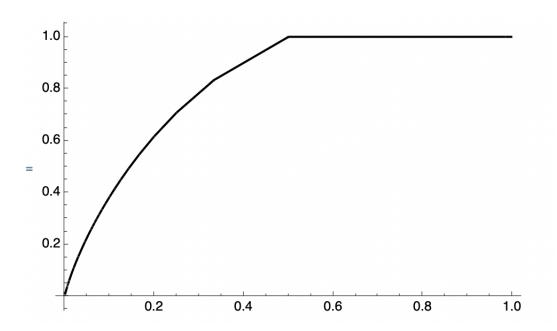
\includegraphics[width=0.7\textwidth]{assets/fig/_page_62_Figure_3.jpeg}
  \caption{$\log(L_{n,k})/n$ 作为 $\gamma = k/n$ 的函数在 $n \to \infty$ 时的边界.}\label{fig:5.0.3}
\end{figure}

\begin{proof}[引理~\ref{lem:5.0.1} 的证明]
我们从第~(1) 部分开始.
由素数定理, $[1, \ldots, n]$ 中的主要项(取对数后)由 $\sum_{p\le n} \log p$ 给出 (即我们只需计算素数而无需计算多重度).
这里的误差项与 $\gamma$ 无关.
因此 $[n - k, \dots, n]$ 的指数渐近速率是通过计算有多少个素数 $p \le n$ 整除 $n - k, \dots, n$ 中的至少一个来给出的.
在这一计数中唯一未出现的素数 $p \le n$ 是那些允许存在 $a \in \mathbf{N}_{>0}$ 使得 $ap < n - k$ 且 $(a + 1)p > n$ 的素数.
对于给定的 $a$, 所涉素数恰好是区间 $(n/(a + 1), (n - k)/a)$ 中的素数.
当且仅当 $a + 1 < 1/\gamma$ 时, 这是一个非空区间; 在这种情况下, 它的长度等于 $n((1 - \gamma)/a - 1/(a + 1))$.
因此, $\log [n - k, \dots, n]$ 等于
\[ n\left(1 - \sum_{a=1}^{\lfloor 1/\gamma \rfloor - 1} \left( \frac{1-\gamma}{a} - \frac{1}{a + 1} \right)\right) + o(n) \]
\[ = n\left(\gamma\left(\sum_{a=1}^{\lfloor 1/\gamma \rfloor - 1} 1/a\right) + 1/(\lfloor 1/\gamma \rfloor)\right) + o(n). \]

注意到根据我们的假设 $\gamma \geq \gamma_0$, 上述求和是一个项数具有一致上界的有限和.
此外, 来自素数定理的误差项得到了均匀控制, 因为它仅被应用于长度和端点在 $n$ 中得到一致控制的区间.

我们现在考虑引理~\ref{lem:5.0.1} 的情况~(2).
第一个断言的精确表述是: 对于任意 $\epsilon > 0$, 存在 $N = N(\epsilon)$ 和 $\delta = \delta(\epsilon)$ 使得对所有 $n > N$ 且 $k < \delta n$, 我们有 $\log L_{n,k} < \epsilon n$.
这是 (1) 的推论.
更确切地, 针对按定义有 $\delta < 1/2$, 对所有 $k < \delta n$, 我们有
\[ L_{n,k} \le L_{n,\delta n} = \exp\left(\left(\sum_{h=1}^{\lfloor 1/\delta \rfloor - 1} \frac{1}{h}\right) \delta n + \frac{n}{\lfloor 1/\delta \rfloor} + o_{\delta}(n)\right) \]
\[ \le \exp\left(\left(\delta(1 + \log(1/\delta)) + (1/\delta - 1)^{-1}\right) n + o_{\delta}(n)\right). \]

注意到 $\lim_{\delta\to 0} \left( \delta(1+\log(1/\delta)) + (1/\delta-1)^{-1} \right) = 0$; 我们选取一个 $\delta = \delta(\epsilon)$ 使得 $\delta(1+\log(1/\delta)) + (1/\delta-1)^{-1} < \epsilon/2$.
对于这个 $\delta$, 由 (1), 存在 $N = N(\delta,\epsilon) = N(\epsilon)$ 使得对 $n > N$, 误差项 $o_{\delta}(n) < (\epsilon/2)n$.
则对于所有 $n > N$ 且 $k < \delta n$, 我们有 $\log L_{n,k} < \epsilon n$.

第二个断言的精确表述是: 对于任意 $\epsilon > 0$, 存在 $N = N(\epsilon)$ 使得对所有 $n > N$ 且所有 $0 \le k \le n$, 我们有
\[ \log L_{n,k} \le \left(\sum_{h=1}^{\lfloor 1/\gamma \rfloor - 1} \frac{1}{h}\right) k + \frac{n}{\lfloor 1/\gamma \rfloor} + \epsilon n. \]

注意到由上述对第一个断言的证明, 存在 $\delta = \delta(\epsilon)$ 使得上述不等式对所有 $n > N_1(\epsilon)$ 且 $k < \delta n$ 成立.
此外, 根据第 (1) 部分取 $\gamma_0 = \delta$, 上述不等式对所有 $n > N_2(\delta, \epsilon) = N_2(\epsilon)$ 成立.
因此, 对于所有 $n > \max\{N_1(\epsilon), N_2(\epsilon)\}$, 所求边界成立.
\end{proof}

以下是上述引理的一个变体.

\begin{lemma}\label{lem:5.0.4}
\quad
\begin{enumerate}
  \item[(1)] 固定 $\gamma_0 \leq \gamma_0' \in (0,1)$. 对于满足 $\gamma_0 \leq k/n$ 且 $\gamma_0 \leq l/n \leq \gamma_0'$ 的 $k, l \leq n$, 大于 $l$ 且在区间 $[n-k, n]$ 内有倍数的素数 $p$ 的乘积 $L_{n,k}^{\geq l}$ 的对数, 在 $n \to \infty$ 时关于 $k, l$ 一致地渐近于
  \[ \left(k\sum_{h=1}^{\lfloor (n-k)/\max(k,l)\rfloor} 1/h\right) + \left(\frac{n}{\lfloor (n+(l-k)^+)/\max(k,l)\rfloor} - l\right)^+ + o(n), \]
  其中 $\alpha^+ := \max(0, \alpha)$, 且约定求和号 $\sum_{h=a}^b$ 遍历该范围内的所有整数, 若范围为空则求和为零.
  
  \item[(2)] 此外, 当 $n \to \infty$ 时, 对于所有 $0 \le k, l \le n$, 我们有
  \[ \log L_{n,k}^{\geq l} \le \left(k \sum_{h=1}^{\lfloor (n-k)/\max(k,l)\rfloor} 1/h\right) + \left(\frac{n}{\lfloor (n+(l-k)^+)/\max(k,l)\rfloor} - l\right)^+ + o(n), \]
  其中误差项关于所有 $k, l$ 是一致的. (若 $k = l = 0$, 则上式右端应理解为 $o(n)$.)
\end{enumerate}
\end{lemma}

\begin{proof}
我们从第 (1) 部分开始.
与引理~\ref{lem:5.0.1} 的证明类似, 在 $[n-k,\ldots,n]$ 中没有倍数的素数 $p \le n$ 是落在 $\bigcup_{a=1}^{\lfloor n/k\rfloor-1} (n/(a+1),(n-k)/a)$ 中的那些.
这里新增加的假设 $p > l$ 蕴含着 $a < (n-k)/l$, 从而
\[ \begin{split} 
& \left( \bigcup_{a=1}^{\lfloor (n-k)/k \rfloor} (n/(a+1), (n-k)/a) \right) \cap (l, n] \\ 
& = \left( \bigcup_{a=1}^{h_0-1} (n/(a+1), (n-k)/a) \right) \cup (\max(n/(h_0+1), l), (n-k)/h_0), 
\end{split} \]
其中 $h_0 = \lfloor (n - k)/\max(k, l) \rfloor$.

根据素数定理, 我们的渐近值由下式给出:
\[ n - l - \left(\sum_{a=1}^{h_0} ((n-k)/a - n/(a+1)) - (\max(n/(h_0+1), l) - n/(h_0+1))\right) + o(n) \]
\[ = k \left( \sum_{a=1}^{h_0} 1/a \right) + \max(n/(h_0 + 1), l) - l + o(n) = k \left( \sum_{a=1}^{h_0} 1/a \right) + (n/(h_0 + 1) - l)^+ + o(n), \]
且
\[ n/(h_0 + 1) = \frac{n}{\lfloor (n-k)/\max(k,l) \rfloor + 1} = \frac{n}{\lfloor (n+(l-k)^+)/\max(k,l) \rfloor}. \]

第二个断言 (2) 的精确表述是: 对于任何 $\epsilon > 0$, 存在 $N = N(\epsilon)$ 使得对所有 $n > N$ 且所有 $0 \le k, l \le n$, 我们有
\[ \log L_{n,k}^{\geq l} \le \left(k \sum_{h=1}^{\lfloor (n-k)/\max(k,l)\rfloor} 1/h\right) + \left(\frac{n}{\lfloor (n+(l-k)^+)/\max(k,l)\rfloor} - l\right)^+ + \epsilon n. \]

由引理~\ref{lem:5.0.1} (2), 存在 $\delta = \delta( \epsilon)$ 使得对于所有 $n > N_1(\epsilon)$ 和所有 $k \le \delta n$, 我们有
\[ \log L_{n,k}^{\geq l} \le \log L_{n,k} < \epsilon n. \]

因此, 我们现在假设 $k > \delta n$.
对于 $l < \min\{\delta, \epsilon/2\}n < k$, 由引理~\ref{lem:5.0.1} (1), 我们有对于 $n > N_2(\delta, \epsilon/2) = N_2(\epsilon)$,
\[ \log L_{n,k}^{\geq l} \le \log L_{n,k} \le \left(k \sum_{h=1}^{\lfloor (n-k)/k \rfloor} 1/h\right) + \frac{n}{\lfloor n/k \rfloor} + (\epsilon/2)n \]
\[ \le \left(k \sum_{h=1}^{\lfloor (n-k)/k \rfloor} 1/h\right) + \left(\frac{n}{\lfloor n/k \rfloor} - l\right)^{+} + \epsilon n, \]
这是所需的边界, 因为在此情况下 $\max(k,l)=k$.
对于 $l > (1-\delta/2)n$, 根据定义, 我们有 $\log L_{n,k}^{\geq l} \le \log L_{n,k}^{\geq (1-\delta/2)n}$.
将 (1) 应用于 $\gamma_0=\delta, \gamma_0'=1-\delta/2$, 存在 $N_3=N_3(\delta)=N_3(\epsilon)$ 使得对所有 $n > N_3$, 我们有
\[
\begin{aligned}
\log L_{n,k}^{\geq (1-\delta/2)n} 
&\le \left(k \sum_{h=1}^{\lfloor (n-k)/\max(k,(1-\delta/2)n)\rfloor} 1/h\right) \\
&\quad + \left(\frac{n}{\lfloor (n+((1-\delta/2)n-k)^+)/\max(k,(1-\delta/2)n)\rfloor} - (1-\delta/2)n\right)^+ + (\epsilon/2)n.
\end{aligned}
\]

注意到第一项为 $0$ (因为 $n-k < (1-\delta/2)n$), 且第二项 $\le n-((1-\delta/2)n \le (\delta/2)n$.
对于上述证明, 我们可以缩小 $\delta$ 使得 $\delta < \epsilon$, 从而以上讨论表明对于所有 $l \ge (1-\delta/2)n$, 我们有所需的边界
\[ \log L_{n,k}^{\geq l} \le \log L_{n,k} \le \epsilon n. \]

现在我们只需考虑 $k \ge \delta n$ 且 $\min\{\delta, \epsilon/2\}n \le l < (1 - \delta/2)n$, 此情况直接由 (1) 得出.
\end{proof}
